\documentclass[11pt, a4paper]{article}

\usepackage[utf8]{inputenc} % Do not change or remove!
%\usepackage[T1]{fontenc} % Do not change or remove
\usepackage[danish]{babel} % Sproget, vi skriver på
\renewcommand\danishhyphenmins{22} % Kun hvis vi skriver på dansk

\usepackage{graphicx} % graphics
\usepackage[dvipsnames]{xcolor}
\usepackage{picture} % insert figures as tex files
\usepackage{epstopdf} % insert eps files
\usepackage{pdfpages} % insert pdf files
\usepackage{microtype} % fixes spaces
\usepackage{tikz}
\usepackage{xspace}
\usepackage{amsmath,amssymb,braket}
\usepackage{gensymb}

% A few handy macros for quantum mechanics notation
\newcommand{\hc}{\; + \; \text{h.c.} \;}
\newcommand{\up}{\uparrow}
\newcommand{\down}{\downarrow}
\newcommand{\sigmap}[1]{\sigma^+_{#1}}
\newcommand{\sigmam}[1]{\sigma^-_{#1}}
\def\te{{\rm e}}
\let\v\vold
\newcommand{\v}[1]{{\bf{#1}}}

%%%%%%%%%%%%%%%%%%%%%%%%% BEGIN DOCUMENT %%%%%%%%%%%%%%%%%%%%%%%%%

\begin{document}

\title{Topologiske isolatorer}
\date{\today}

\author{Niels Jakob Søe Loft \& Kristian Knakkergaard Nielsen}

\maketitle


\section{Krystalstruktur og Blochs sætning}

Faste stoffer er karakteriseret ved, at atomerne er ordnede i et
krystal med en periodisk gitterstruktur. Dette betyder, at en partikel
(fx en elektron), der befinder sig i et faststof, oplever et periodisk
potential, $V(\v r) = V(\v r + \v a)$, hvor $\v a$ er en vektor, der
angiver periodiciteten af krystallen. Den mindste del af systemet, der
udgør det gentagende gitterstruktur, kaldes for enhedscellen. Kendskab
til systemet i enhedscellen (potential, bølgefunktioner,
energiniveauer osv.) beskriver hele systemet. 

Blochs sætning siger, at bølgefunktionerne i et periodisk potential med
periode $a$ kan skrives på formen
\begin{equation}
  \label{eq:bloch}
  \psi_k(x) = e^{ikx} u_k(x) \; ,
\end{equation}
hvor $u_k(x+a) = u_k(x)$ er en periodisk funktion med samme periode
som potentialet og $k$ er bølgetallet. Ovenstående er formuleret i 1 
dimension, men tilsvarende gælder i 2 og 3 dimensioner. Et ækvivalent 
udsagn er, at bølgefunktionen (op til en fasefaktor) er periodisk med 
samme periode (se ligning (1.8) i \cite{gp}).

\begin{itemize}
\item Læs 1.1 i \cite{gp} om Blochs sætning og udled formel~\eqref{eq:bloch}.
\end{itemize}

En anden effekt af et periodisk krystalgitter afspejler sig i
energispektret. I en simpel 1D model kun med nabovekselvirkning er
grundtilstandsenergien givet ved
\begin{equation}
  \label{eq:tb-energi}
  E(k) = E_0 + 2 \gamma \cos ka \; ,
\end{equation}
hvor $E_0 > 0$ og $\gamma < 0$ er konstanter, der afhænger af
materialet.

\begin{itemize}
\item Læs 1.4.1 i \cite{gp} om tætbindingsmodellen og udled
  formel~\eqref{eq:tb-energi}.
\item Sammenlign bølgefunktionen \eqref{eq:bloch} og energispekret
  \eqref{eq:tb-energi} med tilfældene for en fri partikel. Hvilken
  effekt har tilstedeværelsen af det periodiske krystalpotential på
  bølgefunktionen og energispekret?
\end{itemize}

Det fulde energispektrum for et rigtigt materiale indeholder
naturligvis mere end blot ét energibånd. Generelt er
energibåndstrukturen uhyre kompliceret, hvilket I også kan finde
massevis af eksempler på i \cite{gp}. En ikke uvæsentlig del af
faststof går ud på at beregne, analysere og måle båndstrukturer.

\section{Isolatorer og topologiske isolatorer}

Elektronerne i et materiale vil for temperatur $T=0$ besætte
de nederste energitilstande. Fordi elektroner er fermioner, er der kun
plads til én elektron i hver tilstand, så elektronerne besætter
således gradvist tilstandene i energibåndene med stigende energi. Hvis
et energibånd ikke er fuldt besat, kan elektronerne bevæge sig mellem
tilstandene i båndet og lede en elektrisk strøm. Derimod kan
elektronerne i fyldte bånd ikke lede en strøm. Hvis de mest energirige
elektroner akkurat udfylder et bånd, og der er et (forholdsvis stort)
spring op til det næste bånd, vil elektroner ikke springe op i det
tomme bånd, hvor de kan være med til at lede en strøm i materialet. Af
denne årsag kaldes materialer med sådanne båndgap for isolatorer, se
figur~\ref{fig:isolator}.

\begin{figure}[htbp]
  \centering
  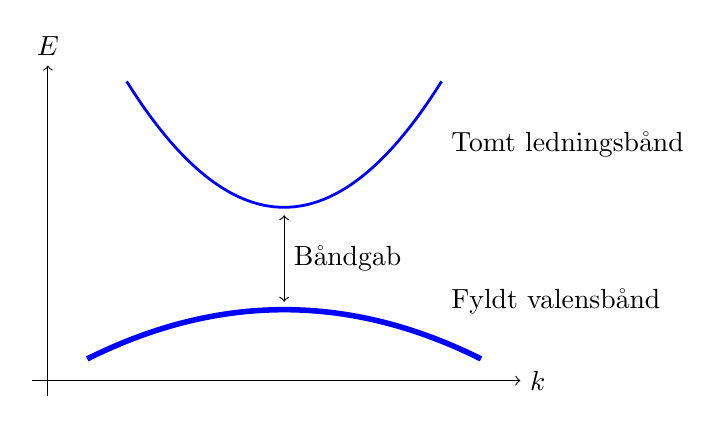
\begin{tikzpicture}
    \draw [->] (-3.2,0) -- (3,0);
    \node [right] at (3,0) {$k$};
    \draw [->] (-3,-.2) -- (-3,4);
    \node [above] at (-3,4) {$E$};

    \draw [color=Blue, line width = 2pt, domain=-2.5:2.5,
    samples=40, smooth]
    plot (\x, {-.1*\x*\x + .9});

    \draw [color=Blue, line width = 1pt, domain=-2:2,
    samples=40, smooth]
    plot (\x, {.4*\x*\x + 2.2});

    \draw [<->] (0,1) -- (0,2.1);
    
    \node [right] at (2,1) {Fyldt valensbånd};
    \node [right] at (2,3) {Tomt ledningsbånd};
    \node [right] at (0,1.55) {Båndgab};
  \end{tikzpicture}  
  \caption{En isolator er karakteriseret ved et båndgab mellem det
    højeste fyldte og nederste ikke-fyldte energibånd.}
  \label{fig:isolator}
\end{figure}


En særlig type af isolatorer kaldes topologiske isolatorer, fordi de 
besidder særlige egenskaber, der kan beskrives vha. den matematiske
diciplin topologi. Topologi handler bl.a. om at karakterisere objekter
vha. tal, der er uændrede under glatte deformationer af objektet. I
denne forstand er en kaffekop og en doughnut ens, men forskellig fra
en fodbold -- her er det antallet af huller i objektet, der er det
invariante topologiske tal, der er uændret under glatte
deformationer. I en topologisk isolator kan energibåndene
karakteriseres vha. lignende topologisk invariante tal. Systemets
topologiske egenskaber, såsom eksistensen af kvantemekaniske
tilstande, der lever på kanten af systemet, er umådeligt robuste,
fordi netop deformationer af systemet kun kan ændre det topologisk
invariante tal i ganske særlige tilfælde. Denne robusthed overfor støj
er en af årsagerne til, at topologiske materialer er blevet spået en
fremtid inden for diverse kvanteteknologier. Opdagelsen af topologiske
materialer og stoffers overgang mellem forskellige topologiske faser
gav i 2016 Thouless, Haldane og Kosterlitz Nobelprisen i fysik.


\section{SSH-modellen}

I dette projekt vil vi i detalje analysere den såkaldte Su-Schrieffer-Heeger (SSH) model. Den blev oprindeligt brugt til at beskrive elektrisk ledning i polymerer af acetylen \cite{ssh}. Først senere fandt man ud af, at denne model er et af de simpleste eksempler på en topologisk isolator. I 2017 lykkedes det i Jacqueline Blochs laboratorium at fremstille modellen eksperimentielt ved hjælp af koblede halvledere \cite{bloch}. Dette vil vi ikke gå i detalje med, men det vil være muligt at vende tilbage til i form af en diskussion af mulige eksperimentelle synteser. 

\subsection{Model, skematisk afbildning og Hamilton-operatoren}

SSH-modellen beskriver fermioner, der hopper rundt i et 1D gitter, bestående af enhedsceller med to skelnelige gitterpunkter: et $A$-punkt og et $B$-punkt. Afstanden mellem enhedscellerne definerer gitterkonstanten $a$. Dette er vist i Fig. \ref{fig.SSH_model}. Ligesom i tætbindingsmodellen er der kun hop mellem $A$- og $B$-punkter, som er naboer. Matrixelementet for at hoppe mellem $A$ og $B$ inden for enhedscellen er $t - \delta t$. For at hoppe uden for enhedscellen er det $t + \delta t$. $\delta t$ beskriver altså hvor forskellige de to matrixelementer er. \\

En fuldstændig basis der beskriver dette system, består således af tilstandene $\{\ket{n, A}, \ket{n, B}\}$ for $1 \leq n \leq N$. Her er $\ket{n, A} = \ket{n}\ket{A}$ en produkttilstand, der beskriver en partikel i enhedscelle $n$ i gitterpunkt $A$. Hvis I er utrygge ved Dirac-notation, så læs eventuelt i \cite{Sakurai}, s. 10-32. 

Vi antager, at de er ortonormale: $\braket{n, I | n', I'} = \delta_{n, n'}\delta_{I, I'}$. Hamilton-operatoren kan da skrives i denne basis som 
\begin{align}
H &= (t - \delta t) \sum_{n = 1}^N\left(\ket{n, A}\bra{n, B} + \ket{n, B}\bra{n, A}\right) \nonumber \\
&+ (t + \delta t) \sum_{n = 1}^N\left(\ket{n + 1, A}\bra{n, B} + \ket{n, B}\bra{n + 1, A}\right),
\label{eq.hamilton}
\end{align}
med $t > 0$. Vi antager desuden (uden tab af generalitet), at $|\delta t| \leq t$. Der er $N$ enhedsceller og vi bruger cykliske randbetingelser. Det sidste betyder, at enhedscelle $n$ og $n + N$ er sammenfaldende. Fysisk antager vi, at kæden er formet som en ring.

\begin{figure}
\begin{center}
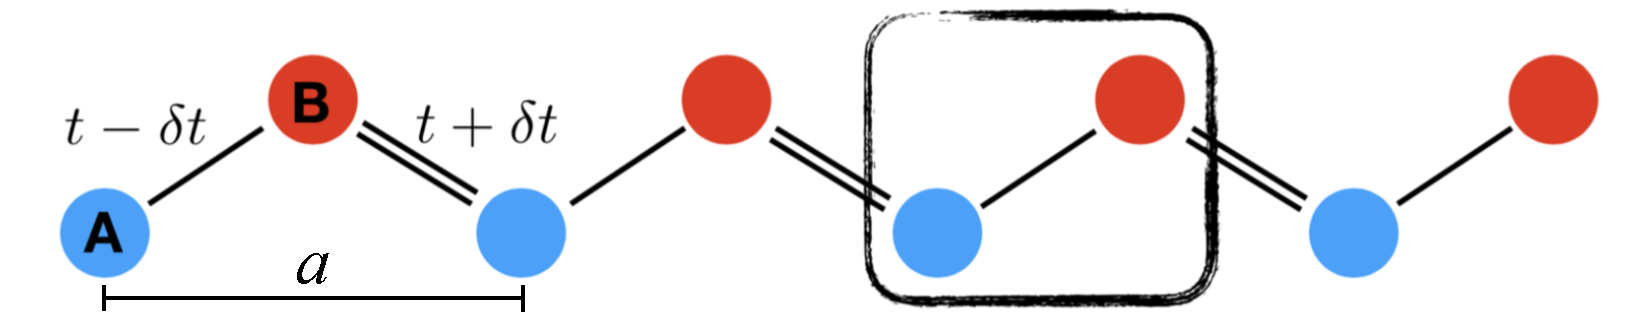
\includegraphics[width=1\textwidth]{SSH_model.pdf} 
\caption{SSH-modellen består af en kæde af f.eks. atomer med to skelnelige gitterpunkter, $A$ og $B$. Enhedscellen består således af ét $A$-punkt og ét $B$-punkt som vist. Enhedscellerne er adskilt af gitterkonstanten $a$. Der er to typer af matrixelementer: mellem $A$ og $B$ inden for enhedscellen: $t - \delta t$, og mellem to forskellige enhedsceller: $t + \delta t$. Alle andre matrixelementer er 0. Herved fremkommer et alternerende mønster indikeret med enkelt- og dobbeltstreger.}
\label{fig.SSH_model}
\end{center}
\end{figure}

\begin{itemize}
	\item Vis, at Hamilton-operatoren \eqref{eq.hamilton} er hermistisk. 

	\item Vis, at Hamilton-operatoren har følgende matrixelementer: 
	\begin{align}
	&\bra{n, B} H \ket{n, A} = \bra{n, A} H \ket{n, B} = t - \delta t, \nonumber \\
	&\bra{n, B} H \ket{n + 1, A} = \bra{n + 1, A} H \ket{n, B} = t + \delta t, \nonumber
	\end{align} 
	for $n = 1, 2, \dots, N$. Overvej at alle andre matrixelementer er 0. 
\end{itemize} 

\subsection{Diagonalisering via Fourier-transformation}
I dette afsnit diagonaliserer vi Hamilton-operatoren. Dvs. vi finder egentilstandene og egenenergierne. Først leder vi efter tilstande $\ket{k}$, der opfylder ligningerne
\begin{equation}
\ket{n} = \frac{1}{\sqrt{N}}\sum_{k} \te^{ik na} \ket{k},
\label{eq.invers_fourier_transform}
\end{equation}
for $1 \leq n \leq N$. Her er $k$ indtil videre blot et reelt tal med samme enhed som et bølgetal (da $ka$ skal være enhedsløs). Ovenstående er ikke rigtig en definition af de nye tilstande, men snarere en ligning vi \textit{ønsker}, de skal opfylde. Vi skal lidt senere se, hvorfor vi gør det. For nu vil vi gerne lære noget mere om, hvad de disse $\ket{k}$-tilstande skal opfylde og finde et eksplicit udtryk for dem.  

\begin{itemize}
	\item Da vi arbejder med cykliske randbetingelser er $\ket{n + N} = \ket{n}$. Vis da, at $\te^{ikNa} = 1$. Overvej, at dette betyder at $k$ kan tage de følgende værdier
	\begin{equation}
	k = l\frac{2\pi}{Na}, 
	\label{eq.k_values}
	\end{equation}
	hvor $l = 0, 1, -1, 2, -2, \dots$ er et heltal. Vi ved dog stadig ikke, hvor mange led der er i $k$-summen.

	\item Vis, at
	\begin{equation}
	\frac{1}{\sqrt{N}}\sum_{n = 1}^N \te^{-ik na}\ket{n} = \sum_{k'}\left[\frac{1}{N}\sum_{n = 1}^N \te^{i(k' - k)na}\right]\ket{k'},
	\end{equation}

	\item Find wikipedia siden for en \textit{geometrisk sum}. Læs om denne og brug det til at vise, at
	\begin{equation}
	\frac{1}{N}\sum_{n = 1}^N \te^{i(k' - k)na} = \delta_{k, k'},
	\label{eq.ortogonalitet}
	\end{equation}
	hvor højresiden er Kroneckers delta. Dvs. denne sum giver et 1-tal, hvis $k' = k$ og ellers giver den $0$. Kan I argumentere mere intuitivt for dette? Vi har da, at
	\begin{equation}
	\ket{k} = \frac{1}{\sqrt{N}}\sum_{n = 1}^N \te^{-ikna}\ket{n}
	\label{eq.fourier_transform}
	\end{equation}
	Overvej, at ligning \eqref{eq.invers_fourier_transform} og \eqref{eq.fourier_transform} er Fourier-transformationer! 

	\item Brug ligning \eqref{eq.fourier_transform} til at vise, at $\ket{k + \frac{2\pi}{a}} = \ket{k}$. 
\end{itemize}
Det sidste punkt viser, at tilstandene kun er veldefineret op til et multiplum af $2\pi / a$. For at have entydige tilstande arbejder vi derfor kun med $k$ i intervallet $(- \pi / a, \pi / a]$. Dette er første Brillouinzone (eller blot Brillouinzonen)! Med andre ord kan $l$ i ligning \eqref{eq.k_values} kun tage værdierne $l = - N / 2 + 1, - N / 2 + 2, \dots, N / 2$. Nu har vi styr på, hvad tilstandene $\ket{k}$ er matematisk. De er defineret ved ligning \eqref{eq.fourier_transform} og \eqref{eq.k_values} med $k$ i intervallet $(- \pi / a, \pi / a]$! \\

Da $k$ fremkommer ved en Fourier-transformation, da $\hbar k$ har samme enhed som impuls og da $\hbar k$ i flere sammenhænge optræder på samme måde som en impuls kaldes $\hbar k$ for \textit{krystalimpulsen}. Vi vender nu tilbage til, hvorfor vi har indført disse nye tilstande. Ved at gange tilstandene $\ket{A}$ og $\ket{B}$ på $\ket{n}$ i ligning \eqref{eq.invers_fourier_transform} får vi

\begin{equation}
\ket{n, A} = \frac{1}{\sqrt{N}}\sum_{k} \te^{ik na} \ket{k, A}, \hspace{0.5cm} \ket{n, B} = \frac{1}{\sqrt{N}}\sum_{k} \te^{ik na} \ket{k, B}. 
\label{eq.k_A_B_tilstande}
\end{equation}

\begin{itemize}
	\item Indsæt udtrykkene i ligning \eqref{eq.k_A_B_tilstande} for $\ket{n, A}$ og $\ket{n, B}$ i Hamilton-operatoren \eqref{eq.hamilton}. Brug igen ligning \eqref{eq.ortogonalitet} og vis, at
	\begin{align}
	H = \sum_k &\left[ \left(t - \delta t + (t + \delta t)\te^{+ika}\right) \ket{k, A}\bra{k, B} \right. \nonumber \\
	& \left. + \left(t - \delta t + (t + \delta t)\te^{-ika}\right) \ket{k, B}\bra{k, A} \right].
	\label{eq.hamilton_krum}
	\end{align}
\end{itemize}

Fordelen ved dette udtryk for $H$ er, at led til forskellige værdier af krystalimpulsen er uafhængige. Derfor kan vi finde egentilstande for hvert $k$! Lad os nu kigge på matrixrepræsentationen $\mathcal{H}_k$ for $H$ for en bestemt krystalimpuls $\hbar k$
\begin{equation}
\mathcal{H}_k = \begin{bmatrix} \bra{k, A} H \ket{k, A} & \bra{k, A} H \ket{k, B} \\ \bra{k, B} H \ket{k, A} & \bra{k, B} H \ket{k, B} \end{bmatrix}.
\end{equation}
Dette er altså i den ordnede basis $\{\ket{k, A}, \ket{k, B}\}$.

\begin{itemize}
	\item Vis, at
	\begin{equation}
	\mathcal{H}_k = \begin{bmatrix} 0 & t - \delta t + (t + \delta t)\te^{-ika} \\ t - \delta t + (t + \delta t)\te^{+ika} & 0 \end{bmatrix}.
	\end{equation}  

	\item Skriv $\mathcal{H}_k$ på formen $\mathcal{H}_k = h_{x, k} \sigma_x + h_{y, k} \sigma_y + h_{z, k} \sigma_z$. Her er $\sigma_x, \sigma_y, \sigma_z$ Pauli-matricer. $h_x, h_y, h_z$ definerer en vektor. Vis, at
	\begin{equation}
	\mathbf{h}_k = \begin{bmatrix} h_{x, k} \\ h_{y, k} \\ h_{z, k} \end{bmatrix} = \begin{bmatrix}  t - \delta t + (t + \delta t)\cos(ka) \\ (t + \delta t)\sin(ka) \\ 0 \end{bmatrix}.
	\end{equation}

	\item Vinklen mellem $h_{x, k}$ og $h_{y, k}$ er azimuthalvinklen $\phi_k$. Denne er altså givet ved de implicitte formler
	\begin{equation}
	\cos(\phi_k) = \frac{h_{x, k}}{|\mathbf{h}_k|}, \hspace{0.5cm} \sin(\phi_k) = \frac{h_{y, k}}{|\mathbf{h}_k|}.
	\label{eq.phik_definition}
	\end{equation}
	Denne viser sig at gemme på den topologiske invariant, som vi skal se på i næste afsnit. Vær derfor sikker på, at I forstår hvad denne vinkel/fase er. Lav eventuelt en tegning med $h_x$ på $x$-aksen, $h_y$ på y-aksen, tegn vektoren $\mathbf{h}$ og vinklen $\phi$. 

	\item Vis, at
	\begin{equation}
	\mathcal{H}_k = |\mathbf{h}_k| \begin{bmatrix} 0 & \te^{-i \phi_k} \\ \te^{+i \phi_k} & 0 \end{bmatrix}.
	\label{eq.H_k_final}
	\end{equation}
\end{itemize}
Vi kan nu finde egentilstande og egen-energier ved at finde egenvektorer og egenværdier til $\mathcal{H}_k$. Det viser sig, at der for hvert $k$ er 1 grundtilstand og 1 exciteret tilstand beskrevet ved egenvektorerne $\mathbf{u}_{\pm, k}$ med tilhørende egenværdier $E_{\pm, k}$

\begin{align}
\mathbf{u}_{-, k} &= \frac{1}{\sqrt{2}}\begin{bmatrix} 1 \\ -\te^{i\phi_k} \end{bmatrix}, \hspace{0.5cm} E_{-, k} = - |\mathbf{h}_k|. \nonumber \\
\mathbf{u}_{+, k} &= \frac{1}{\sqrt{2}}\begin{bmatrix} 1 \\ +\te^{i\phi_k} \end{bmatrix}, \hspace{0.5cm} E_{+, k} = + |\mathbf{h}_k|. \nonumber
\end{align}


\begin{itemize}
	\item Tjek, at $\mathcal{H}_k \mathbf{u}_{\pm, k} = E_{\pm, k} \mathbf{u}_{\pm, k}$. 

	\item $E_{\pm, k} = \pm |\mathbf{h}_{\pm, k}|$ er altså egenenergierne for hvert $k$. Båndgabet for SSH-modellen er altså $\Delta E = 2\; {\rm min}_k |\mathbf{h}_k|$. Tegn disse energier som funktion af $k$ (i første Brillouinzone) for forskellige værdier af $\delta t$ og marker $\Delta E$. Prøv f.eks. $\delta t = - t / 2, \; 0, \; t / 2$. 

	\item Er der en værdi af $\delta t$, hvor $\Delta E = 0$? 
\end{itemize}

Vha. egenvektorer til $\mathcal{H}_k$ kan vi nu konstruere de endelige egentilstande, $\ket{\psi_{\pm}, k}$. Explicit med $\mathbf{u}_{-, k} = (u_{1-, k}, u_{2-, k})$ og tilsvarende for $+$ er

\begin{align}
	\ket{\psi_-, k} &= u_{1-, k}^* \ket{k, A} + u_{2-, k}^* \ket{k, B} = \frac{1}{\sqrt{2}}\left[\ket{k, A} - \te^{-i \phi_k}\ket{k, B} \right], \nonumber \\
	\ket{\psi_+, k} &= u_{1+, k}^* \ket{k, A} + u_{2+, k}^* \ket{k, B} = \frac{1}{\sqrt{2}}\left[\ket{k, A} + \te^{-i \phi_k}\ket{k, B} \right].
	\label{eq.eigenstates}
\end{align}

Vi har altså fundet egentilstandene til Hamilton-operatoren. Den nuværende analyse fokuserer på \textit{det indre} af systemet. Dette kaldes "bulk" på engelsk. I afsnittet om kanttilstanden skal vi se, at hvis vi åbner ringen, så kæden har en ende og dermed en kant, kan der snige sig en ekstra tilstand ind, som er eksponentielt lokaliseret på denne kant.   

\begin{itemize}
	\item Omskriv Hamilton-operatoren til
	
	\begin{equation}
	H = \sum_k |\mathbf{h}_k|\left[\te^{i\phi_k}\ket{k, A}\bra{k, B} + \te^{-i\phi_k}\ket{k, B}\bra{k, A}\right].
	\label{eq.Hamilton_final}
	\end{equation}

	\item Ved at bruge ligning \eqref{eq.eigenstates} og \eqref{eq.Hamilton_final} tjek da, at $H\ket{\psi_\pm, k} = E_{\pm, k}\ket{\psi_\pm, k}$. 

\end{itemize}

Ekstra opgave:

\begin{itemize}
	\item Ved at bruge at $\braket{m | n, A} = \delta_{n, m} \ket{A}$ vis, at 
	\begin{equation}
	\braket{m| \psi_{\pm, k}} = \frac{1}{\sqrt{2N}}\te^{-ikma}\left(\ket{A} \pm \te^{-i\phi_k}\ket{B}\right). 
	\end{equation}
	Dette giver en forbindelse til Blochs sætning. Kan I se hvordan? \textit{Hint}: I ovenstående er $x = ma$ $x$-koordinaten. Har det samme form som $\psi_k(x) = \te^{-ikx} u_k(x)$?
\end{itemize}
Vi er nu klar til at definere og studere den topologiske invariant. 

\subsection{Den topologiske invariant}
Den topologiske invariant for SSH-modellen er det såkaldte omdrejningstal $\mathcal{W}$ (på engelsk: \textit{winding number}). Dette er defineret ud fra fasen $\phi_k$ vi stødte på i foregående afsnit

\begin{equation}
\mathcal{W} = \frac{1}{2\pi} \int_{-\pi / a}^{\pi / a} \frac{d\phi_k}{dk} dk. 
\label{eq.definition_omdrejningstal}
\end{equation}
I denne formel betragter vi krystalimpulsen som en kontinuert variabel. Overvej at dette er ok, når $N \gg 1$. I figur \ref{fig.omdrejning} vises, hvordan $\phi_k$ ændrer sig som funktion af $k$ for to værdier af $\delta t$. I næste afsnit viser vi, hvorfor dette er en invariant. For nu bruger vi blot ovenstående som en definition og beregner den som funktion af $\delta t$. 


\begin{figure}
\begin{center}
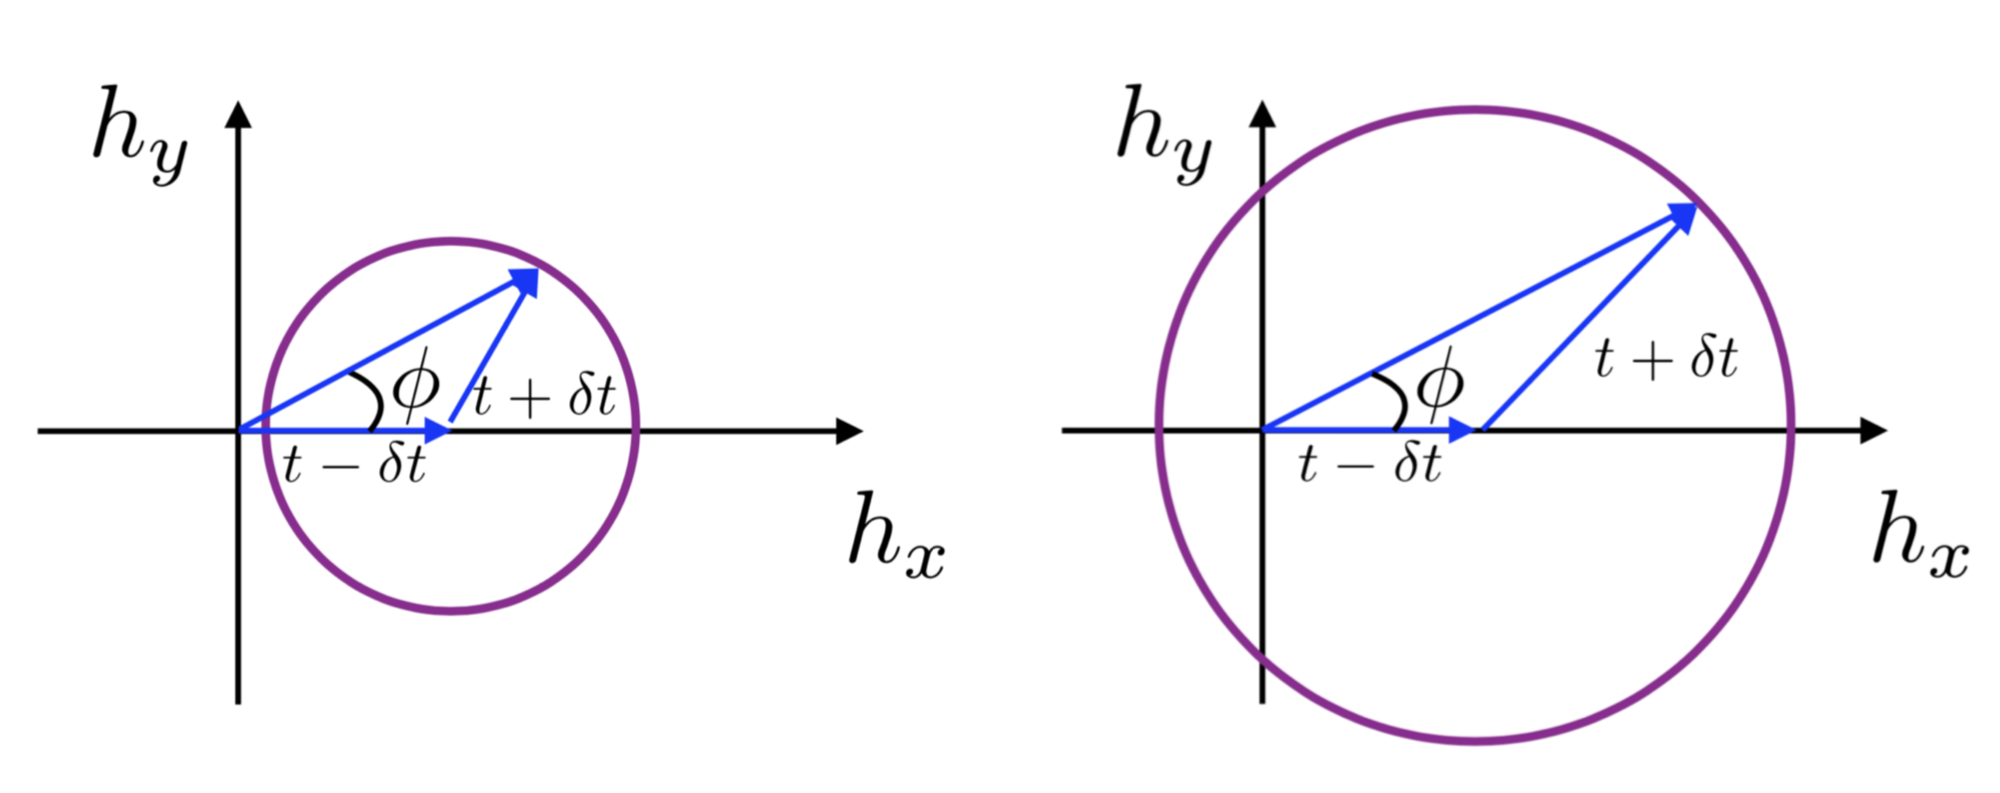
\includegraphics[width=1\textwidth]{omdrejning.png} 
\caption{Skitse af $h_x, h_y$ og vinklen $\phi_k$ for to værdier af $\delta t$. Til venstre er $\delta t < 0$. Til højre er $\delta t > 0$. }
\label{fig.omdrejning}
\end{center}
\end{figure}

\begin{itemize}
\item Lav en tegning som i figur \ref{fig.omdrejning} af vektoren $\mathbf{h}_k$. 

\item Hvad er $\mathcal{W}$ på de to tegninger? Er den forskellig for $\delta t < 0$ og $\delta t > 0$? 
\end{itemize}

De to ovenstående punkter giver en grafisk løsning af integralet i \eqref{eq.definition_omdrejningstal}, der giver

\begin{equation}
\mathcal{W} = \left\{\begin{matrix} 0, & \delta t < 0. \\ 1, & \delta t > 0. \end{matrix} \right.
\label{eq.resultat_omdrejning}
\end{equation}
Dette viser, at $\mathcal{W}$ ændrer sig diskontinuert i $\delta t = 0$. 


\begin{itemize}
	\item Hvad er båndgabet $\Delta E$ for $\delta t = 0$? 
\end{itemize}


Ekstra opgaver:
\begin{itemize}
	\item Ved at bruge $\tan(\phi_k) = h_{y, k} / h_{x, k}$ vis da, at

	\begin{equation}
	\frac{d\phi}{dk} = a \frac{(t + \delta t)^2 + (t - \delta t)(t + \delta t)\cos(ka)}{(t + \delta t)^2 + (t - \delta t)^2 + 2 (t - \delta t)(t + \delta t)\cos(ka)}. 
	\end{equation}
	\textit{Hint}: skriv først $\phi_k = {\rm arctan}(h_{y, k} / h_{x, k}) + C$, hvor $C$ er en konstant. Differentier dette udtryk og reducér. Dette er lidt svært, så hæng i! 

	\item Vi kan bruge dette udtryk til at beregne $\mathcal{W}$ eksplicit. Plot $d\phi / dk$ for $\delta t = -t, -t / 2, 0, t / 2, t$. 

	\item Indsæt $\delta t = - t, 0, t$ i $d \phi / dk$. Hvad er $\mathcal{W}$ i disse tre tilfælde? Passer det med figur \ref{fig.omdrejning}? 
\end{itemize}


\subsection{Symmetri og topologi}
I dette afsnit definerer vi, hvad en topologisk faseovergang er. Vi kigger derefter på, hvordan omdrejningstallet fra foregående afsnit er tilknyttet dette. Det er et ret svært afsnit, hvor I skal lære en del nye begreber, så vær tålmodige. \\

Når vand går fra is til væske, kalder vi det en faseovergang. Den flydende fase, væsken, er translations-invariant. Det betyder, at hvis jeg står et sted i væsken og flytter mig (eller \textit{translaterer} mig), ser det ud på samme måde som før. Væsken er altså invariant under min translation. 

I den faste fase, isen, er det ganske anderledes. Is er et krystal. Specifikt er det ikke ens overalt. Hvis f.eks. jeg starter ved et gitterpunkt, sidder der et atom. Men går jeg halvvejs til det næste atom, er der slet ikke noget. Translations-invariansen er brudt! Det er et eksempel på et såkaldt spontant symmetribrud, som ofte sker, når man køler noget ned. Det beskriver vand og mange andre materialers faser, samt meget eksotiske faser som et Bose-Einstein kondensat og superledende materialer. I alle disse tilfælde bliver en symmetri brudt ved et bestemt punkt. I dette punkt er den såkaldte \textit{frie energi} ens for de to faser. Dette lærer I mere om i Statistisk Fysik! For vand brydes translationsinvariansen ved $T = 0\degree {\rm C}$, når det går fra flydende til fast form. \\

\textit{Topologiske} faseovergange er anderledes! Der er stadig en energiforskel, som er 0 lige ved faseovergangen. I dette tilfælde er det båndgabet $\Delta E$. Men i modsætning til ovenstående er en bestamt fase ikke defineret ved, om den har en vis symmetri, som en anden fase ikke har. Tværtimod sker der slet ikke et symmetribrud i en topologisk faseovergang. Idéen er altså, at når vi ændrer en bestemt variabel lukker båndgabet $\Delta E$ sig ved et bestemt punkt. Det fører til følgende definition af topologiske faser. \\

\textit{Topologisk faser er tilstande, der har et båndgab, som ikke bryder nogen symmetrier spontant, og som ikke kan konverteres til hinanden uden at lukke båndgabet.} \\

For SSH-modellen er $\delta t$ vores variabel, og båndgabet lukker sig i $\delta t = 0$. I dette punkt så vi også, at omdrejningstallet $\mathcal{W}$ ændrede sig fra $0$ til $1$. Vi skal nu se, at hvis systemet overholder en bestemt symmetri, \textit{skal} båndgabet lukke sig, hvis omdrejningstallet ændrer sig fra $0$ til $1$. Derfor er systemet i to forskellige topologiske faser for $\mathcal{W} = 0$ og $\mathcal{W} = 1$. Et sådant tal der er konstant i en bestemt topologisk fase, og som kun ændrer sig, hvis båndgabet lukker sig, kaldes en \textit{topologisk} invariant. \\

Denne type af topologiske faser, som er beskyttede af en symmetri, kaldes \textit{symmetri-beskyttede topologiske faser}. Der findes endnu mere eksotiske systemer og tilhørende tilstande, hvis topologiske tilstande slet ikke afhænger af nogen symmetrier. Dem vil vi dog ikke komme nærmere ind på. Symmetrien vi hentyder til i denne sammenhæng, ser således ud
\begin{equation}
S = P_A - P_B = \sum_{n = 1}^N \left[\ket{n, A}\bra{n, A} - \ket{n, B}\bra{n, B}\right]. 
\label{eq.subgitter_symmetri}
\end{equation}
Her er $P_A = \sum_{n = 1}^N \ket{n, A}\bra{n, A}$ en projektion på $A$-gitterpunkter, tilsvarende for $P_B$. 

\begin{itemize}
	\item Vis, at $P_A H P_A = 0 = P_B H P_B$. 

	\item Overvej, at $P_A + P_B = \mathbb{I}$. Altså er summen af projektionerne identitetsoperatoren.

	\item Brug ovenstående til at vise, at $SHS = - H$. \textit{Hint}: Skriv $S = P_A - P_B$ og skriv $SHS$ ud i fire led. Brug derefter punkt 1 og 2 ovenfor.  
\end{itemize}

En symmetri på denne form, hvor $SHS = -H$, kaldes for en subgitter-symmetri (på engelsk: sublattice symmetry). Deraf bogstavet $S$. 

\begin{itemize}
	\item Vis, at $S^2 = \mathbb{I}$. \textit{Hint}: Brug, at identiteten kan skrives som $\mathbb{I} = \sum_{n = 1}^N \left[\ket{n, A}\bra{n, A} + \ket{n, B}\bra{n, B}\right]$.  

	\item Vis, at $SH = -HS$. 

	\item Antag, at $\ket{\psi_E}$ er en egentilstand med energi $E$: $H \ket{\psi_E} = E \ket{\psi_E}$. Vis, at $H(S\ket{\psi_E}) = -E(S\ket{\psi_E})$. Altså er $S\ket{\psi_E}$ en egentilstand med energi $-E$. Dette viser, at der til enhver tilstand med energi $E$ findes en tilhørende tilstand med energi $-E$. Med andre ord er energispektret symmetrisk omkring 0! Dette er formentlig grunden til, at $S$ kaldes for en symmetri. 

	\item Vis eksplicit for de fundne egentilstande tidligere, at $S\ket{\psi_{+, k}} = \ket{\psi_{-, k}}$. Dvs. de fundne egentilstande er forbundet af $S$.  
\end{itemize}

Vi ønsker nu at studere, hvilke restriktioner på $H$ det giver at antage, at $S$ er en symmetri. Til dette formål antager vi nu, at $H$ har en noget mere generel form, hvor $\mathcal{H}_k$ skrives som
\begin{equation}
\mathcal{H}_k = h_{x, k}\sigma_x + h_{y, k}\sigma_y + h_{z, k}\sigma_z. 
\label{eq.general_Hamilton}
\end{equation}
Man kan vise, at enhver $2\times 2$ matrix af interesse kan skrives på denne form. Man kan herved også vise, at $\mathcal{H}_k$, og den tilhørende Hamilton $H$, beskriver en generel gitter-periodisk Hamilton i 1D med to energibånd. 

\begin{itemize}
	\item Fourier-transformér $S$ til $k$-rum: 

	\begin{equation}
	S = \sum_k \left[\ket{k, A}\bra{k, A} - \ket{k, B}\bra{k, B}\right]. 
	\label{eq.S_i_krum}
	\end{equation}

	\item Beregn matrix-repræsentationen $\mathcal{S}$ af $S$ i basen $\{\ket{k, A}, \ket{k, B}\}$. \textit{Resultat}: $S = \sigma_z$, den tredje Pauli-matrix. 

	\item Omskriv $S$ og $H$ til følgende
	\begin{align}
	S &= \sum_k \begin{bmatrix}\ket{k, A} & \ket{k, B} \end{bmatrix} \mathcal{S} \begin{bmatrix}\bra{k, A} \\ \bra{k, B} \end{bmatrix}, \nonumber \\
	H &= \sum_k \begin{bmatrix}\ket{k, A} & \ket{k, B} \end{bmatrix} \mathcal{H}_k \begin{bmatrix}\bra{k, A} \\ \bra{k, B} \end{bmatrix}, 
	\end{align}
	hvilket altså eksplicit indeholder $\mathcal{S}, \mathcal{H}_k$. Her skal $\begin{bmatrix}\ket{k, A} & \ket{k, B} \end{bmatrix}$ forstås som en rækkevektor indeholdende tilstandene $\ket{k, A}, \ket{k, B}$. 

	\item Vis, at $SH = -HS \Leftrightarrow \mathcal{S}\mathcal{H}_k = -\mathcal{H}_k\mathcal{S}$. Dette er ikke så nemt. Spørg endelig, hvis det er for svært. 
\end{itemize}

Sidste punkt viser, at vi blot kan analysere operatorerne i termer af matrixrepræsentationerne for hvert $k$. 

\begin{itemize}
	\item Vis, at $\mathcal{S}\mathcal{H}_k = -\mathcal{H}_k\mathcal{S} \Leftrightarrow h_{z,k} = 0$ for alle $k$. Det betyder, at vektoren $\mathbf{h}$ altid ligger i $(h_x, h_y)$-planen. 

	\item Overvej, at så længe systemet overholder symmetrien $S$, og så længe båndgabet er åbent ($\Delta E \neq 0$), så er omdrejningstallet $\mathcal{W}$ et heltal. 

	\item Overvej yderligere, at omdrejningstallet kun kan ændre sig, hvis $\Delta E = 0$ krydses.

	\item Overvej, at hvis systemet ikke overholder $S$, dvs. hvis $h_{z, k} \neq 0$, så kan vi godt ændre omdrejningstallet fra $0$ til $1$, \textit{uden} at båndgabet lukker!
\end{itemize}

De sidste tre punkter ovenfor viser, at omdrejningstallet er en topologisk invariant, \textit{hvis} systemet overholder symmetrien $S$. 

\subsection{Kanttilstanden}
I dette afsnit kigger vi på, hvilken fysisk konsekvens det har, at systemet kan være i to forskellige topologiske faser. Vi konstruerer i denne sammenhæng eksplicit en ekstra tilstand for $\delta t > 0$, som er eksponentielt lokaliseret på kanten af systemet. Dette forbinder den topologiske fase med tilstedeværelsen af en kanttilstand. \\

For at analysere opførslen af materialet nær en kant, åbner vi kæden, og lader den have en ende mod venstre. Således kan Hamilton-operatoren skrives
\begin{align}
H &= (t - \delta t) \sum_{n = 1}^\infty\left(\ket{n, A}\bra{n, B} + \ket{n, B}\bra{n, A}\right) \nonumber \\
&+ (t + \delta t) \sum_{n = 1}^\infty\left(\ket{n + 1, A}\bra{n, B} + \ket{n, B}\bra{n + 1, A}\right).
\label{eq.hamilton_aaben}
\end{align}
Der er altså ikke nogen enhedsceller til venstre for $n = 1$. Lad nu
\begin{equation}
\ket{\psi} = \sum_{m = 1}^{\infty}\left[a_m \ket{m, A} + b_m \ket{m, B} \right]. 
\label{eq.kanttilstand_ansatz}
\end{equation}
Dette er en generel ansatz for den ønskede kanttilstand.

\begin{itemize}
	\item Vi ønsker at tilføje en tilstand til det allerede fundne energispektrum med $E_{\pm, k}$ og samtidig stadig overholde symmetrien $S$. Overvej, at hvis vi skal finde en enkelt tilstand, så må den have energi $E = 0$. \textit{Hint}: energispektret er symmetrisk omkring 0!

	\item Vi antager altså, $H \ket{\psi} = 0$. Brug dette til at vise, at
	\begin{align}
	0 &= (t - \delta t)\sum_{n = 1}^\infty\left[a_n\ket{n, B} + b_n\ket{n, A}\right] \nonumber \\
	&+ (t + \delta t)\sum_{n = 1}^\infty\left[a_{n + 1}\ket{n, B} + b_n\ket{n + 1, A}\right].
	\label{eq.kanttilstand_2}
	\end{align}

	\item Brug ortogonaliteten af tilstandene $\ket{m, A}, \ket{m, B}$ til at vise, at
	\begin{align}
	0 &= (t - \delta t)a_m + (t + \delta t)a_{m + 1} \nonumber \\
	0 &= (t - \delta t)b_{m + 1} + (t + \delta t)b_m.
	\label{eq.kanttilstand_3}
	\end{align}
	\textit{Hint}: Brug $\bra{m, A}$ og $\bra{m, B}$ ind på ligning \eqref{eq.kanttilstand_2}. 

	\item Ved at virke med $\bra{1, A}$ ind på ligning \eqref{eq.kanttilstand_2}, vis da at $(t - \delta t)b_1 = 0$. Dvs. $b_1 = 0$!

	\item Brug anden lighed i \eqref{eq.kanttilstand_3} til at vise, at $b_m = 0$ for alle $m$. 

	\item Brug nu første lighed i \eqref{eq.kanttilstand_3} til først at vise, at $a_{m + 1} = - a_m (t - \delta t)/(t + \delta t)$. Vis derefter, at
	\begin{equation}
	a_{m + 1} = \left(-\frac{t - \delta t}{t + \delta t}\right)^{m} a_1.
	\label{eq.kanttilstand_4}
	\end{equation}

	\item Lad $c = \ln \frac{t + \delta t}{t - \delta t}$. For hvilket fortegn af $\delta t$, er $c > 0$? Vis, at $a_m = (-1)^{m-1} \te^{-(m - 1)c}$. Overvej, at $\ket{\psi}$ \textit{ikke} er normerbar for $\delta t < 0$. 
\end{itemize}

Det sidste punkt ovenfor viser, at vi ikke kan konstruere den ønskede kanttilstand for $\delta t < 0$. Det kan vi til gengæld for $\delta t > 0$. Explicit har vi altså nu

\begin{equation}
\ket{\psi} = \sum_{n = 1}^{\infty} (-1)^{n - 1}\te^{-(n - 1)c}a_1 \ket{n, A} = - \te^{c}a_1 \sum_{n = 1}^{\infty} (-1)^n\te^{-n c}\ket{m, A}. 
\label{eq.kanttilstand_naesten_faerdig}
\end{equation}

\begin{itemize}
	\item Overvej, at ligning \eqref{eq.kanttilstand_naesten_faerdig} viser, at $\ket{\psi}$ er eksponentielt lokaliseret på kanten, dvs. ved $n = 1$. 

	\item Normér kanttilstanden, dvs. sæt $\braket{\psi|\psi} = 1$, og vis at 
	\begin{equation}
	1 = e^{2c}|a_1|^2 \sum_{n = 1}^{\infty} e^{-2nc}. 
	\end{equation}

	\item Brug formlen for en geometrisk række: $\sum_{n = 0}^{\infty} r^n = \frac{1}{1 - r}$ til at vise
	\begin{equation}
	\sum_{n = 1}^{\infty} e^{-2nc} = \sum_{n = 0}^{\infty} e^{-2nc} - 1 = \frac{1}{\te^{2c} - 1}. 
	\end{equation}

	\item Antag, at $a_1$ er positiv og reel. Vis da, at
	\begin{equation}
	a_1 = \left(\frac{\te^{2c} - 1}{\te^{2c}}\right)^{1/2} = \frac{\sqrt{1 - \te^{-2c}}}{\te^{c}}
	\end{equation}

\end{itemize}

Vi får da endelig, at
\begin{equation}
\ket{\psi} = \sqrt{1 - \te^{-2c}}\sum_{n = 1}^{\infty} (-1)^{n - 1} \te^{-nc}\ket{n, A}. 
\label{eq.kanttilstand_faerdig}
\end{equation}
med $c = \ln \frac{t + \delta t}{t - \delta t}$. 

\begin{itemize}
	\item Hvad sker der, hvis $\delta t \to t$? 

	\item Hvad sker der, hvis $\delta t \to 0$? 
\end{itemize}

Vi ser altså, at hvis $\mathcal{W} = 1$, så er der en kanttilstand. Hvis $\mathcal{W} = 0$, er der ikke en! Dette forbinder en bulk-effekt, omdrejningstallet der kun afhænger af tilstandene $\ket{\psi_\pm, k}$, til en kanteffekt, tilstedeværelsen af en kanttilstand. Det betyder også, at vi kan forudsige, om der vil være en kanttilstand udelukkende ved at analysere bulk (eller det indre) af systemet. Dette er et kraftfuldt værktøj til at finde systemer, der har interessante kanttilstande. F.eks. har en gas af elektroner i et 2D-plan med et ortogonalt magnetfelt, kanttilstande langs randen, som kan lede strøm uden modstand.  I dette system er det uhyre svært rent faktisk at konstruere tilstandene eksplicit. Ikke desto mindre kan vi forudsige, at de må være der, og vi kan forudsige, at de leder strøm uden modstand. \\


Da denne strøm viser sig at være kvantiseret, kan det bruges til meget præcist at måle strøm. Dette blev udnyttet i forberedelsesarbejdet til at lave en ny udgave af SI-enhedssystemet, det internationale system af måleenheder, som forventes at træde i kraft i 2019. Man kan nemlig bruge denne kvantiserede strøm til meget præcist at måle Plancks konstant $h$. Efter disse meget præcise målinger har man nu \textit{defineret} Plancks konstant til at have en bestemt værdi. På denne vis er en række naturkonstanter nu \textit{definerede} størrelser, heriblandt altså Plancks konstant og ligeledes lysets hastighed i vacuum. Disse kan så bruges til at konvertere til de enheder, vi er mere vant til at bruge, en meter for længde, et sekund for tid og et kilogram for masse. Dette erstatter den noget forældede definition af et kilogram som massen af et bestemt standardlod i platin og iridium konstrueret tilbage i 1889. Selvom denne legering er meget modstandsdygtig over for ændringer over tid, er det selvfølgelig ikke perfekt. Derudover vil massen af loddet også ændres en anelse, når det er i kontakt med luft, da luftmolekyler kan sætte sig på overfladen. Da man har flere lodder i samme legering udover standarden, har man da også kunnet påvise, at disse andre lodders masse over tid varierer relativt til standarden. Det betyder altså, at selve definitionen af masse har ændret sig over tid (i størrelsesordenen nogle mikrogram). Dette er selvfølgelig ganske utilfredsstillende og har nu ført til helt nye definitioner, der er uafhængige af sådanne standarder. 

\newpage
\begin{thebibliography}{9}
  \bibitem{Sakurai} J.J. Sakurai: {\it Modern Quantum Mechanics}, Revised edition, 1994
  \bibitem{gp}
    G. Grosso \& G. P.  Parravicini: {\it Solid State Physics}, 2nd ed.,
    Academic Press (2014)
  \bibitem{gb} G. M. Bruun: {\it Lecture Notes for Solid State Physics II} (2016)
  \bibitem{ssh} W. P. Su, J. R. Schrieffer \& A. J. Heeger: {\it Phys. Rev.} \textbf{42}, 1698 (1979) 
  \bibitem{bloch} P. St--Jean, V. Goblotm E. Galopin, A. Lemaitre, T. Ozawa, L. Le Gratiet, I. Sagnes, J. Bloch \& A. Amo: {\it Nature Photonics} \textbf{11}, 651-656 (2017)
\end{thebibliography}


\end{document}




